%==============================================================================
% This is a document for writing the final report for EE260 project. 
%
% It uses the NeurIPS (formerly NIPS) style. When making changes, please refer 
% to the style file and example given (../nips_style/neurips_2020.tex)

% Please leave comments as you see it necessary; it will help others 
% who also need to modify the document. 
% -JBU
%==============================================================================

\documentclass{article}
% if you need to pass options to natbib, use, e.g.:
%     \PassOptionsToPackage{numbers, compress}{natbib}
% before loading neurips_2020

% ready for submission
% \usepackage{neurips_2020}

% to compile a preprint version, e.g., for submission to arXiv, add add the
% [preprint] option:
%     \usepackage[preprint]{neurips_2020}

% to compile a camera-ready version, add the [final] option, e.g.:
%     \usepackage[final]{neurips_2020}

% to avoid loading the natbib package, add option nonatbib:
     \usepackage[final, nonatbib]{./../nips_style/neurips_2020}

\usepackage[utf8]{inputenc} % allow utf-8 input
\usepackage[T1]{fontenc}    % use 8-bit T1 fonts
\usepackage{hyperref}       % hyperlinks
\hypersetup{
    colorlinks=true,
    linkcolor=blue,
    filecolor=magenta,      
    urlcolor=cyan,
}

\usepackage{url}
\urlstyle{same}            % simple URL typesetting
\usepackage{booktabs}       % professional-quality tables
\usepackage{amsfonts}       % blackboard math symbols
\usepackage{nicefrac}       % compact symbols for 1/2, etc.
\usepackage{microtype}      % microtypography

\usepackage{graphics}
\usepackage{graphicx} % For including and formatting image files
\usepackage{multirow}
\usepackage{longtable}
\usepackage{epsfig}
\usepackage{epstopdf}

\usepackage{amsmath, mathrsfs, dsfont}
\usepackage{amssymb}
\usepackage{amsfonts}
\usepackage{bm}


\usepackage{cite}
\usepackage{verbatim}

\usepackage{amscd}
\usepackage{color}

\usepackage{rotating}


\usepackage[font=footnotesize]{caption}
%\usepackage[caption=false,font=footnotesize]{subfig}
\usepackage[font=footnotesize]{subcaption}

%\usepackage{mathptmx}
\usepackage[11pt]{moresize}
\usepackage{flushend}
\usepackage[stable]{footmisc}

\usepackage{algorithmicx}
\usepackage[ruled]{algorithm}
\usepackage{algpseudocode}
\usepackage{algpascal}
\usepackage{algc}
\usepackage{enumitem}

%\usepackage{lipsum,multicol}

\usepackage[vcentermath]{youngtab} % For typesetting Young Tableaux

%---------
\usepackage{arydshln}

%-----------------------------------------%
% Define custom symbols
\newcommand{\BoldA}				{ \mathbf{A} }
\newcommand{\Bolda}				{ \mathbf{a} }
\newcommand{\BoldB}				{ \mathbf{B} }
\newcommand{\Boldb}				{ \mathbf{b} }
\newcommand{\BoldC}				{ \mathbf{C} }
\newcommand{\Boldc}				{ \mathbf{c} }
\newcommand{\BoldD}				{ \mathbf{D} }
\newcommand{\BoldE}				{ \mathbf{E} }
\newcommand{\Bolde}				{ \mathbf{e} }
\newcommand{\BoldF}				{ \mathbf{F} }
\newcommand{\BoldG}				{ \mathbf{G} }
\newcommand{\g}					{ \mathbf{g} }
\newcommand{\BoldH}				{ \mathbf{H} }
\newcommand{\Boldh}				{ \mathbf{h} }
\newcommand{\BoldI}				{ \mathbf{I} }
\newcommand{\I}					{ \mathbf{I} }
\newcommand{\BoldJ}				{ \mathbf{J} }
\newcommand{\BoldK}				{ \mathbf{K} }
\newcommand{\Boldk}				{ \mathbf{k} }
\newcommand{\BoldM}				{ \mathbf{M} }
\newcommand{\Boldm}				{ \mathbf{m} }
\newcommand{\BoldN}				{ \mathbf{N} }
\newcommand{\Boldn}				{ \mathbf{n} }
\newcommand{\BoldO}				{ \mathbf{O} }
\newcommand{\BoldP}				{ \mathbf{P} }
\newcommand{\Boldp}				{ \mathbf{p} }
\newcommand{\BoldQ}				{ \mathbf{Q} }
\newcommand{\Boldq}				{ \mathbf{q} }
\newcommand{\BoldR}				{ \mathbf{R} }
\newcommand{\R}					{ \mathbf{R} }
\newcommand{\Boldr}				{ \mathbf{r} }
\newcommand{\BoldS}				{ \mathbf{S} }
\newcommand{\BoldT}				{ \mathbf{T} }
\newcommand{\BoldU}				{ \mathbf{U} }
\newcommand{\Boldu}				{ \mathbf{u} }
\newcommand{\BoldV}				{ \mathbf{V} }
\newcommand{\Boldv}				{ \mathbf{v} }
\newcommand{\BoldW}				{ \mathbf{W} }
\newcommand{\BoldX}				{ \mathbf{X} }
\newcommand{\Boldx}				{ \mathbf{x} }
\newcommand{\BoldY}				{ \mathbf{Y} }
\newcommand{\Boldy}				{ \mathbf{y} }
\newcommand{\BoldZ}				{ \mathbf{Z} }
\newcommand{\Boldz}				{ \mathbf{z} }

\newcommand{\CC}{\mathbb{C}}
\newcommand{\NN}{\mathbb{N}}
\newcommand{\QQ}{\mathbb{Q}}
\newcommand{\RR}{\mathbb{R}}
\newcommand{\ZZ}{\mathbb{Z}}

\newcommand{\0}					{ \boldsymbol{0} }
\newcommand{\1}					{ \boldsymbol{1} }

\newcommand{\dtheta}			{ \delta\boldsymbol{\theta} }
\newcommand{\noiseg}			{ \mathbf{n}_{g} }
\newcommand{\noisewg}			{ \mathbf{n}_{{\omega}g} }
\newcommand{\noisea}			{ \mathbf{n}_{a} }
\newcommand{\noisewa}			{ \mathbf{n}_{{\omega}a} }
\newcommand{\Boldomega}			{ \boldsymbol{\omega} }
\newcommand{\Boldnu}			{ \boldsymbol{\nu} }
\newcommand{\BoldGamma}			{ \boldsymbol{\Gamma} }
\newcommand{\Boldgamma}			{ \boldsymbol{\gamma} }
\newcommand{\Boldkappa}			{ \boldsymbol{\kappa} }
\newcommand{\BoldPhi}			{ \boldsymbol{\Phi} }
\newcommand{\Boldphi}			{ \boldsymbol{\phi} }
\newcommand{\Boldpi}			{ \boldsymbol{\pi} }
\newcommand{\Boldrho}			{ \boldsymbol{\rho} }
\newcommand{\Boldell}			{ \boldsymbol{\ell} }
%\newcommand{\0}					{ \boldsymbol{0} }
\newcommand{\Bolddelta}			{ \boldsymbol{\delta} }
\newcommand{\BoldTheta}			{ \boldsymbol{\Theta} }
\newcommand{\Boldtheta}			{ \boldsymbol{\theta} }
\newcommand{\BoldSigma}			{ \boldsymbol{\Sigma} }
\newcommand{\Boldsigma}			{ \boldsymbol{\sigma} }
\newcommand{\Boldeps}			{ \boldsymbol{\epsilon} }
\newcommand{\Boldmu}			{ \boldsymbol{\mu} }
\newcommand{\Boldeta}			{ \boldsymbol{\eta} }
\newcommand{\Boldzeta}			{ \boldsymbol{\zeta} }
\newcommand{\Boldlambda}		{ \boldsymbol{\lambda} }
\newcommand{\BoldLambda}		{ \boldsymbol{\Lambda} }
\newcommand{\Boldchi}			{ \boldsymbol{\chi} }

\newcommand{\E}					{\mathrm{E}}
\newcommand{\Var}				{\mathrm{Var}}
\newcommand{\Cov}				{\mathrm{Cov}}
\newcommand\norm[1]{\lVert#1\rVert}

\def\I{{\mathrm I}}
\def\II{{\mathrm{II}}}
\def\III{{\mathrm{III}}}

\def\SS{{\mathbb S}}
\def\o{{\omega}}
\def\O{{\Omega}}
\def\L{{\Lambda}}
\def\t{{\theta}}
\def\l{{\lambda}}
\def\vt{{\vartheta}}
\def\p{{\prime}}
\def\pa{{\partial}}
\def\d{{\delta}}
\def\b{{\beta}}
\def\a{{\alpha}}
\def\e{{\varepsilon}}
\def\beq{\begin{equation}}
\def\eeq{\end{equation}}

\newcommand{\Z}{{\mathbb Z}}
\newcommand{\R}{{\mathbb R}}
\newcommand{\Q}{{\mathbb Q}}
\newcommand{\C}{{\mathbb C}}
\newcommand{\D}{{\mathbb D}}
\newcommand{\T}{{\mathbb T}}
\newcommand{\E}{{\mathbb E}}
\newcommand{\N}{{\mathbb N}}
\newcommand{\PP}{{\mathbb P}}
\newcommand{\HH}{{\mathbb H}}

\newcommand{\CA}{{\mathcal A}}
\newcommand{\CC}{{\mathcal C}}
\newcommand{\CD}{{\mathcal D}}
\newcommand{\CE}{{\mathcal E}}
\newcommand{\CF}{{\mathcal F}}
\newcommand{\CG}{{\mathcal G}}
\newcommand{\CB}{{\mathcal B}}
\newcommand{\CH}{{\mathcal H}}
\newcommand{\CI}{{\mathcal I}}
\newcommand{\CL}{{\mathcal L}}
\newcommand{\CM}{{\mathcal M}}
\newcommand{\CN}{{\mathcal N}}
\newcommand{\CX}{{\mathcal X}}
\newcommand{\CP}{{\mathcal P}}
\newcommand{\CS}{{\mathcal S}}
\newcommand{\CY}{{\mathcal Y}}
\newcommand{\CZ}{{\mathcal Z}}
\newcommand{\CU}{{\mathcal U}}
\newcommand{\CK}{{\mathcal K}}
\newcommand{\CO}{{\mathcal O}}
\newcommand{\CJ}{{\mathcal J}}
\newcommand{\Tau}{\mathcal{T}}


\title{Few Shot Object Detection Using Fine-tuning}

\author{% Please fill in your info
  Jean-Bernard Uwineza 
  %\thanks{Use footnote for providing further information
  %  about author (webpage, alternative address)---\emph{not} for acknowledging
  %  funding agencies.} 
  \\
  %Department of Electrical Engineering \\
  University of California, Riverside\\
  Riverside, CA 92501 \\
  \texttt{buwineza@ee.ucr.edu} \\
  \And
  Chetan Reddy Mudireddy \\
  University of California, Riverside \\
  Riverside, CA 92501 \\
  \texttt{cmudi001@ucr.edu} \\
  \AND
  %
  Om Shankar Ohdar \\
  University of California, Riverside \\
  Riverside, CA 92501 \\
  \texttt{oohda001@ucr.edu} \\
  \And
  %
  Sayak Nag \\
  University of California,Riverside \\
  Riverside, CA 92501 \\
  \texttt{snag005@ucr.edu} \\
  %
  \And
  Vikarn Bhakri \\
  University of California, Riverside \\
  Riverside, CA 92501 \\
  \texttt{vbhak001@ucr.edu} \\
}

\begin{document}

\maketitle

\begin{abstract} 

Despite the recent overwhelming success of deep convolutional neural networks in  
object detection, they  still require large amounts of annotated examples per category  
to perform well. Few-shot object detection aims to detect rare object categories that 
often have only a few examples, and might not be present in training examples. 
Most approaches have focused on meta-learning techniques such as feature re-weighting, 
or feature re-generation. 
This report explores a technique of finetuning only the last layer of the detection network. 
It is shown that this  gives overwhelmingly better results despite being relatively simple. 
The network was trained on base classes of PASCAL VOC, and COCO datasets containing general classes. 
We additionally show that the model is able to generalize by evaluating it on novel 
classes from the KITTI dataset. 
\end{abstract}

\subsection{Some rules for collaboration} % TO BE REMOVED BEFORE SUBMISSION 

\begin{itemize}
  \item DO NOT delete text you did not write, unless the person who wrote it asks you. 
  If you have issues with some of the text, discuss with the author first. 
 
  \item Commit and push to GitHub often. This helps others staying updated. 

  \item Apply other common sense rules of collaboration.

\end{itemize}

\section{Introduction}
{\color{magenta}
Few-shot learning has received significant interest in the past few years, 
but mainly for the tasks of classification and rarely for object detection. 
In computer vision, the task of object detection is more challenging since the detector 
not only has to perform recognition of the different kinds of objects present,
it also has to localize them. This is already a challenging task that relies heavily 
on the availability of massive amounts of labeled training data. Now when a new data-point 
is obtained belonging to a novel category, adapting the model becomes a very difficult 
task especially when the new category contains a few samples. Recently, meta learning techniques 
have been proposed for adapting deep models to novel categories. However, they are not easily 
extendable to the task of object detection. Take for example the Matching \cite{VinyalsBLKW16} 
and Prototypical Networks \cite{snell2017prototypical}, building prototypes of objects is 
much more difficult than building prototype of the categories. Another approach that is being 
explored by researchers is to provide ways to fine-tune the detection layers of 
deep models to adapt to the new categories \cite{wang2020frustratingly}.


In this project we aim to do a comparative study of meta-learning and fine-tuning approaches 
towards object detection. We aim to experiment on benchmark datasets such as 
COCO \cite{LinMBHPRDZ14} and PASCAL \cite{Everingham10} and also extend these approaches 
towards 3D object detection with the KITTI dataset \cite{Geiger2013IJRR}.

In addition, we plan on examining how many shots are necessary to reach comparable accuracy relative to 
conventional detection approaches. To this end, we will attempt to develop a metric that assesses
the model's knowledge, and requests additional labeled examples if it has not reached a certain accuracy. 
This will allow us to further compare the performance of the two approaches. 
} 

\section{Existing Approaches}
\subsection{General Detectors}

There are many approaches to the general object detection problem. The most prominent and successful ones use
deep convolutional neural networks (Deep CNNs). A series of related detectors in
\cite{girshick2014rich,girshick2015fast,ren2015faster} began with R-CNN, a network which uses pre-trained CNNs 
to classify region proposals \cite{girshick2014rich}. The proposals are generated using  a method of 
selective search introduced in \cite{uijlings2013selective}. Fast R-CNN \cite{girshick2015fast} added a
region-of-interest (RoI) pooling layer to extract regional features directly from convolutional maps. 
Faster R-CNN \cite{ren2015faster} introduced an entire region proposal network (RPN) to speed region proposal.

In the pursuit of yet more detection speed and simplicity, there is another group of detectors which 
forgoes region proposal. The YOLO series of detectors begins with \cite{redmon2016yolo}, 
a detector which uses a single convolutional network to directly perform class and bounding box predictions. 
Incremental improvements  are introduced in \cite{redmon2017yolo9000,redmon2018yolov3}. 
Since these methods do not require a separate classifier for each region, they are simpler and faster than 
proposal-based methods.


Since few-shot detection in not mainly concerned with speed, it borrows many techniques from 
proposal-based approaches. Specifically, RoI layers and RPN networks will be used in the approach 
explored in this paper (see Section \ref{two-stage-finetuning}).

\begin{figure}[]
  \centering
  \begin{minipage}{1\textwidth}
  \centering
  % \fbox{
  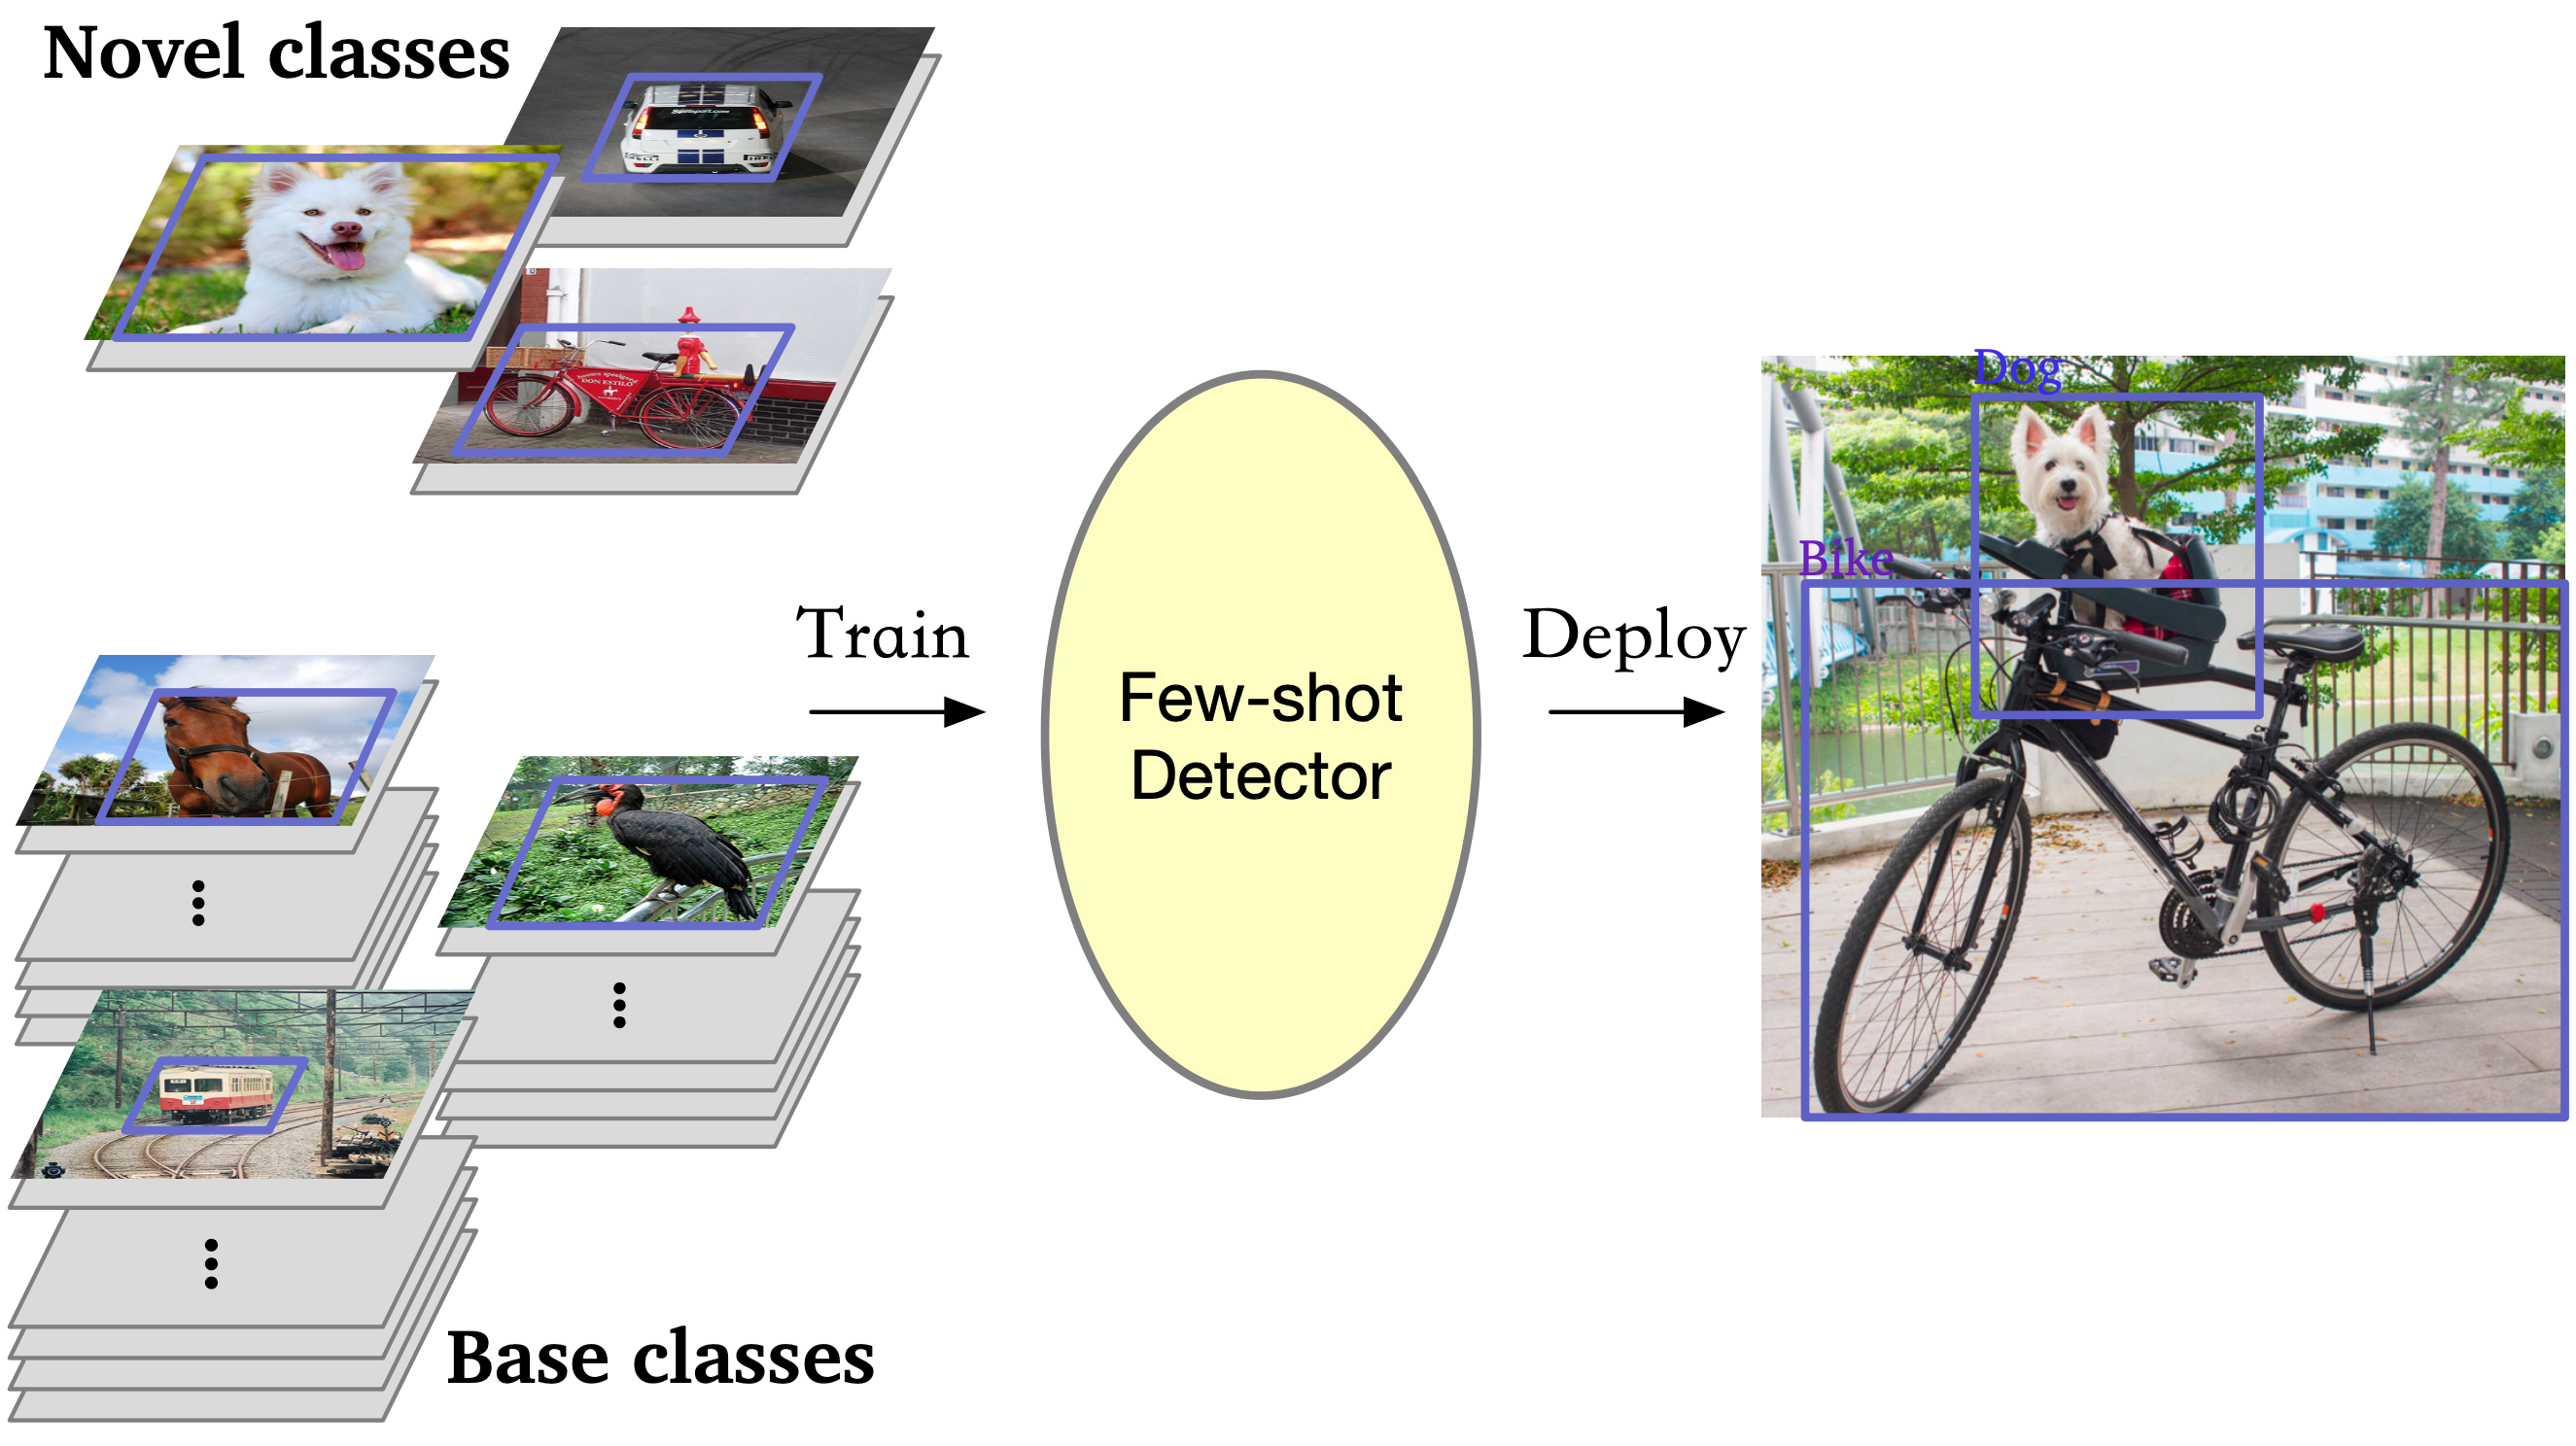
\includegraphics[width=0.79\textwidth, height=0.27\textheight]{./../../figures/fs_det/fs-det.png}
  % }
  \end{minipage}
\caption{A typical few-shot object detection process. Base classes contain abundant 
training examples per object category, while novel class only have a few examples 
per category. The few-shot detector must generalize well enough to detect novel objects 
from only a few examples.}
\label{fs-det}
\end{figure}

\subsection{Few-shot Detectors}
Early work on few-shot learning used Bayesian inference as an attempt to generalize knowledge 
learned from a pre-trained model \cite{fei2006one}. Currently, meta-learning approaches are the most popular.
Particularly, a subclass called metric learning performs detection using a similarity metric. 
Matching networks in \cite{VinyalsBLKW16} attempts to learn the similarity between the target image and 
a small set of labeled images. This idea is extended by Prototypical Networks \cite{snell2017prototypical} 
by using a linear classifier instead of nearest-neighbor for each class. 
All the above are for the classification task. 

For detection, \cite{kang2019few} defines a setting in which two kinds of training data are available: 
\textit{base classes} and \textit{novel classes}. This is shown in Figure \ref{fs-det}. 
Base classes have abundant labeled samples, while 
novel classes have only a limited number of samples. The job of the detector is to use knowledge 
of base classes to  learn how to detect novel objects in a test setting that includes both base and novel classes. 
This is motivated partly by the fact that large-scale object detection datasets (such as 
PASCAL VOC and MSCOCO) only contain a limited number of object categories. However, these datasets can be 
used in training as base classes to support the introduction of novel classes. 

In meta-learning, a \textit{meta-leaner} is used to acquire class-level meta-knowledge and help the model 
generalize to novel classes through various techniques such as feature re-weighting \cite{kang2019few}
or class-specific feature generation \cite{wang2019meta}. The meta-learner trains on a small set of support 
images with full annotations of target objects, and is often jointly trained with the detector using episodic
training, in which each episode comprises of $N$ supporting objects a set of few query images \cite{VinyalsBLKW16}. 
The training is also divided into two stages; in the first stage the model is only trained on 
base classes, and in the second stage the model is fine-tuned on a support set of a few examples 
of the novel classes  and a small subset of the base classes. 

The approach explored herein adopts this two-stage training regime, but it gets rid of memory inefficiency 
of episodic training. \cite{wang2020frustratingly}. Instead, the fine-tuning is only done 
on the last layers of the network with a normal batch training scheme (See Section \ref{two-stage-finetuning}). 

\section{Few-shot Finetuning}

\subsection{Problem Definition}
Suppose there is  a set of base classes $C_b$ with \textit{sufficiently many} training examples and a set $C_n$ 
of novel classes with only $K$ examples per class (in this paper $K \leq 10$ always). 
The few-shot datasets used herein are balanced, meaning that for each novel class there are $K$ annotated examples.
When $K$ examples are used in finetuning, we call it a $k$-shot detection. 
Denote the set of training images as $\mathcal{X}$ and their corresponding labels as $\mathcal{Y}$. 
A detection dataset $\mathcal{D} = \{ (x,y), ~ x \in \mathcal{X}, ~ y \in \mathcal{Y} \}$, where $x$ 
is the input image and $y= \{(c_i, \bm 1_i) \}_{i=1}^N$ denotes the categories $c \in  C_b \cup C_n$ and 
bounding box coordinates $\1 $ of the $N$ instances of the object in the image $x$. 

In \cite{VinyalsBLKW16} and \cite{snell2017prototypical}, as is usually used in few-shot learning, 
the authors use $N$-way $K$-shot regime for evaluation, where $N$ is the number of training examples, 
and $K$ is the number of classes in the training set. 
In this paper, the detector model is evaluated on a test set that includes base and novel classes
to optimize the detection accuracy as measured by mean average precision (mAP) of both novel and base classes.


\begin{figure}[h]
  % \centering
  \begin{minipage}{0.47\textwidth}
  % \fbox{
  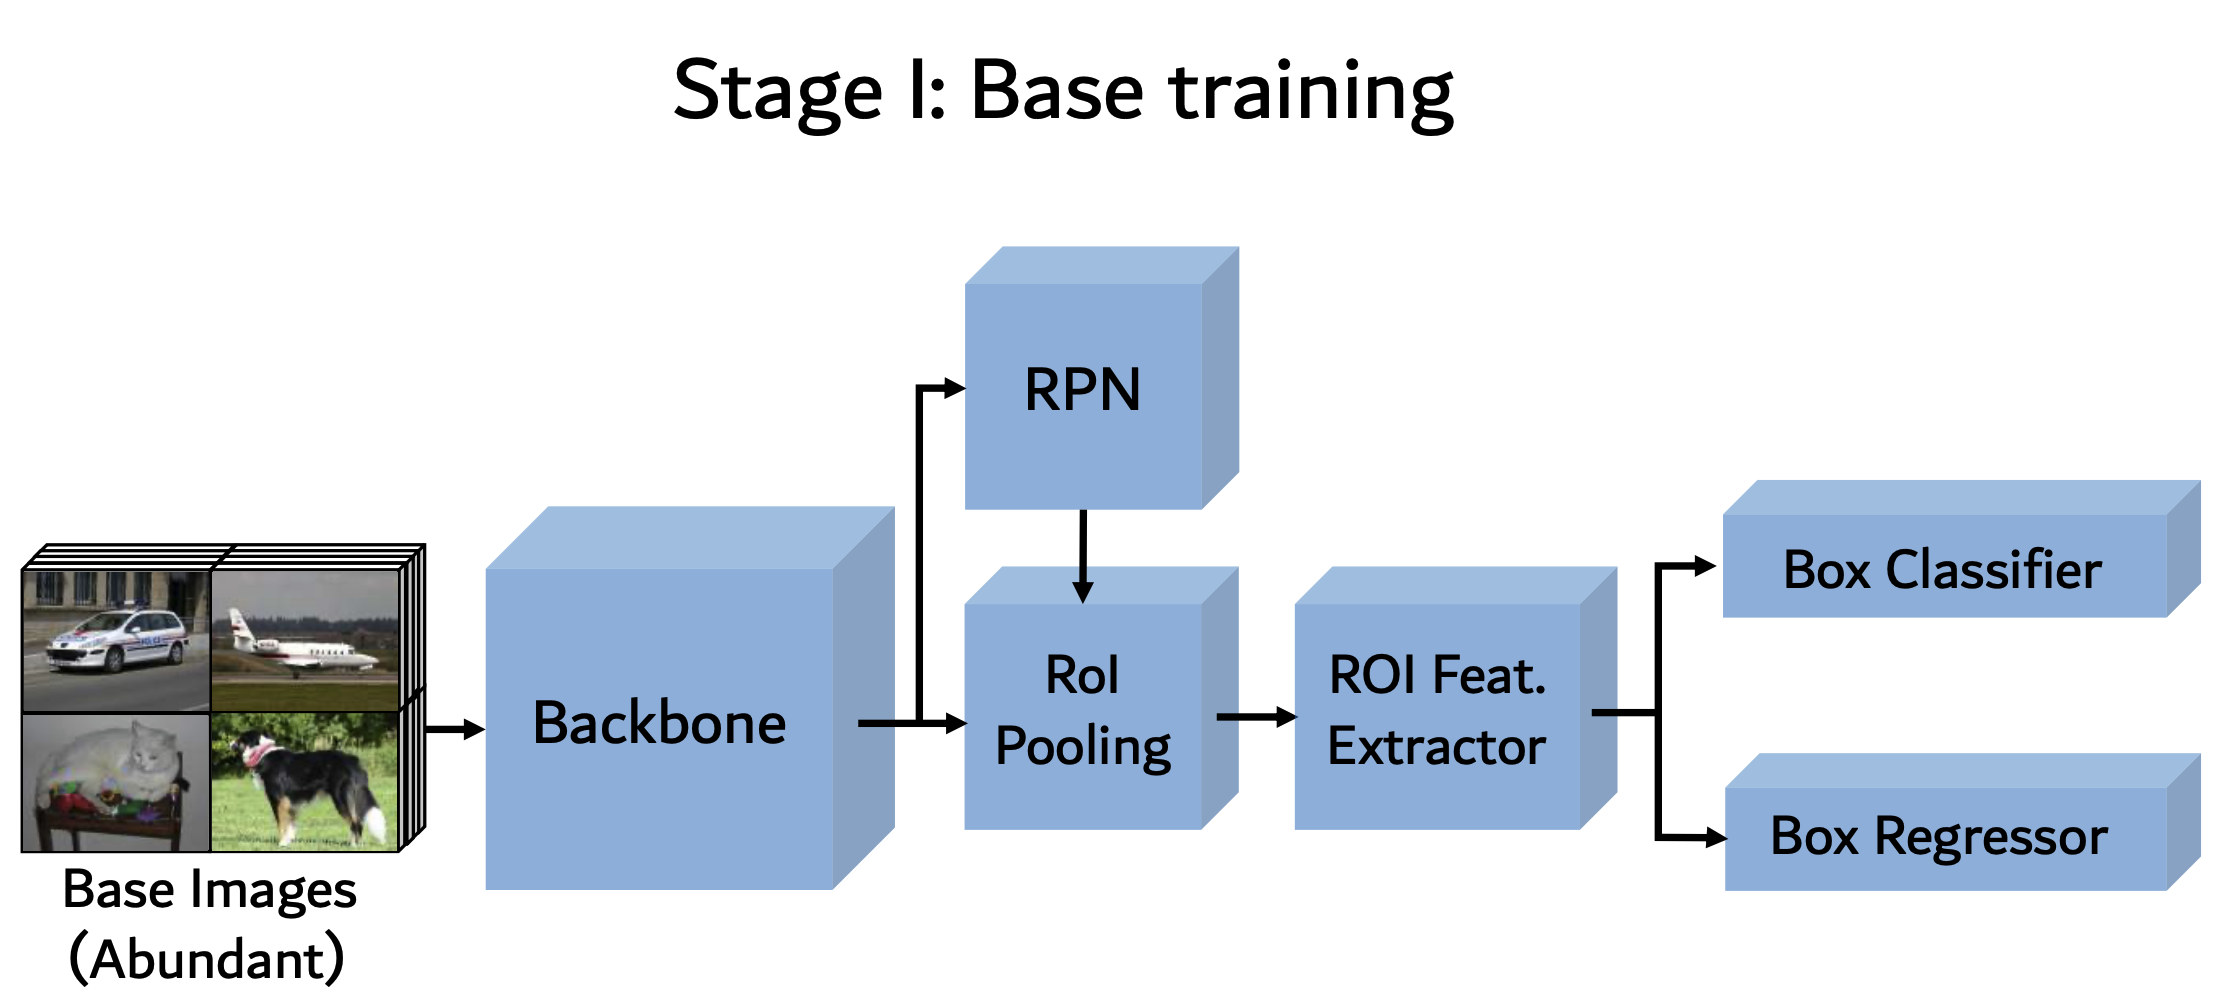
\includegraphics[width=\textwidth, height=0.17\textheight]{./../../figures/fs_det/s1_finetuning.png}
  % }
  \subcaption{Stage I}
  \label{stage-1-finetuning}
  \end{minipage}
  %
  \begin{minipage}{0.47\textwidth}
  % \fbox{
  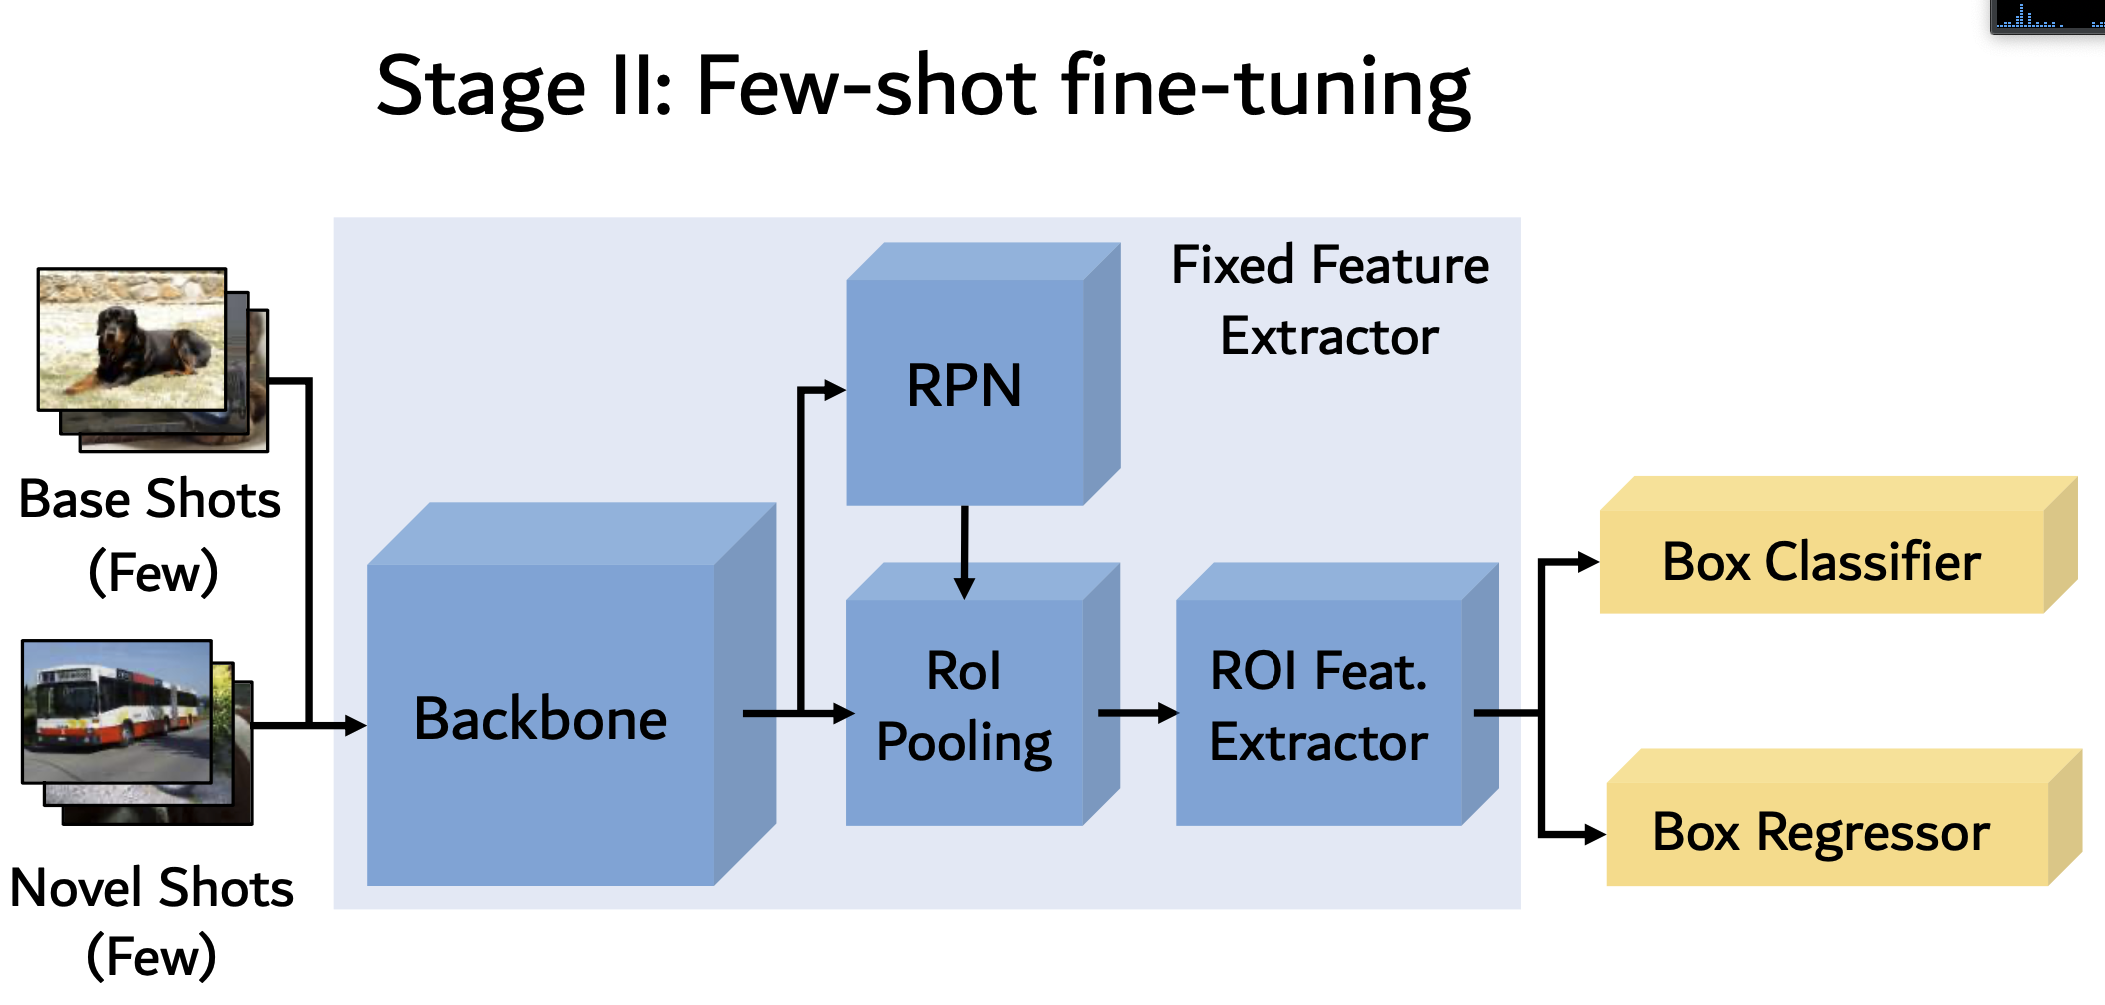
\includegraphics[width=\textwidth, height=0.17\textheight]{./../../figures/fs_det/s2_finetuning.png}
  % }
  \subcaption{Stage II}
  \label{stage-2-finetuning}
  \end{minipage}
  \caption{Stage I \& II of  the finetuning process. Figure courtesy of Wang et al. }
  \label{finetuning}
\end{figure}

\subsection{Two-stage Finetuning} \label{two-stage-finetuning}
In a two-stage process, we adopt the simple finetuning approach of \cite{wang2020frustratingly}. 
This approach builds on Faster R-CNN \cite{ren2015faster}, a popular two-stage object detector model. 
The approach is pictured in Figure \ref{finetuning}.  
Figure \ref{stage-1-finetuning} shows that the Faster R-CNN model has three main components, namely, 
the backbone, the Region Proposal Network (RPN), and the two-layer fully-connected network as a 
Region of Interest (RoI) feature extractor.  
The backbone used in this paper is the ResNet architecture \cite{he2016deep}, but it could be any other 
architecture such as the VGG16. The ResNet was chosen because it is relatively easier to optimize,
hence potentially easier to adapt to novel classes. 
In addition to Faster R-CNN model, henceforth denoted $\mathcal{F}$, the approach also uses a box 
classifier $\mathcal{C}$ for classifying objects into different classes and a box regressor $\mathcal{R}$
to predict the bounding boxes. 

The main intuitive assumption is that $\mathcal{F}$ is able to transfer the feature function 
$\mathcal{F}(x)$ learned from base classes to 
novel classes. In other words, $\mathcal{F}$ is class-agnostic. This leads to the main contribution of 
\cite{wang2020frustratingly}: a suggestion that when introducing novel classes, it matters 
little to retrain $\mathcal{F}$. Instead, only the the box classifier $\mathcal{C}$ and regressor $\mathcal{R}$
need to be finetuned on the examples of novel classes since the features of base classes learned with $\mathcal{F}$ 
will easily transfer to novel classes. In this way, feature representation learning and box 
prediction learning are separated into two stages, as shown in Figure \ref{finetuning}.

\textbf{Stage I: Base Training. } 
The feature  extractor and the box predictor are trained on a dataset containing 
base classes, $C_b$. The training loss function \cite{ren2015faster} is 
\begin{equation}
  L = L_{\mathcal{F}} + L_{\mathcal{C}} + L_{\mathcal{R}}. 
  \label{loss_func}
\end{equation}
The $L_{\mathcal{F}}$ loss is obtained from the output of the RPN network, hence, it helps distinguishing 
background from foreground. The $L_{\mathcal{C}}$ loss is a cross-entropy loss of the box classifier, and 
$L_{\mathcal{R}}$ is the robust loss function (smoothed $L_1$) of the box regressor. More details on $L$ can be
found in \cite{ren2015faster} and \cite{girshick2015fast}. 

\textbf{Stage II: Finetuning. }
In this stage, a small training set containing $K$ examples per class, with both base and novel classes. 
Using a smaller learning rate\footnote{The finetuning learning rate is reduced by at least 20 times compared 
to base training learning rate. In our experiments, it was reduced from $2\cdot10^{-2}$ to $1\cdot10^{-3}$.} 
and the same loss function as in \eqref{loss_func}, the box classifier 
and regressor are initialized with random weights for the novel classes and are finetuned 
while the feature extractor $\mathcal{F}$ is fixed and unmodified. 


\subsection{Euclidean Distance-based Similarity}
The weight matrix $W \in \RR^{d \times c}$ of the box classifier $\mathcal{C}$ can be expressed as 
  $W = [w_1, w_2, \dots, w_c]$ 
where the row-vector  $w_c \in \RR^d$ is the weight vector of each class.  
Recent works (such as \cite{VinyalsBLKW16,chen2019closer,qi2018low,gidaris2018dynamic}) have proposed 
box classifiers based on cosine similarity. The output of the classifier is a scaled similarity score matrix 
of the input features and the weight vectors of the classes. Specifically
\begin{equation}
  s_{ij} = \frac{\alpha \mathcal{F}(x)_i^\top w_j}{\| \mathcal{F}(x)_i \| \|w_j\|},
\end{equation}
where $\alpha$ is the scaling factor\footnote{In \cite{wang2020frustratingly}, a fixed value 
of $\alpha = 20$ was used.}. 
Cosine similarity is attractive because it offers feature normalization which reduces the 
variance between classes and improves detection accuracy for novel classes \cite{wang2020frustratingly}. 

We now propose a different similarity score, in which the Euclidean distance between the 
input features and class weight vectors is passed through the Softmax function. Specifically
\begin{equation}
  s_{ij} = \frac{e^{-\|\mathcal{F}(x)_i - w_j\|_2^2}}{\sum_{j} e^{-\|\mathcal{F}(x)_i - w_j\|_2^2}}.
\end{equation}
The Euclidean distance is one of the simplest distance metrics, and it has been shown in \cite{snell2017prototypical} 
to outperform cosine similarity scores. 
We extend this metric and find that this similarity score provides a stronger kind of feature normalization 
which should help the model adapt well when introducing novel classes. 

\section{Experimental Results}
\subsection{Experimental Setup}
The network architecture has been provided in section 3.2. All models were trained using SGD with a minibatch size of 16, the momentum of 0.9, and a weight decay of 0.0001. A learning rate of 0.02 is used during base training and 0.001 during few-shot fine-tuning. For base training, the model was trained for 20 epochs in total with early stopping for COCO and Pascal-VOC and then fined-tuned for the novel categories for 10 epochs. For KITTI, the PASCAL-VOC base feature detector was fixed and only the last layers we fine-tuned for 20 epochs.

For the PASCAL VOC dataset, its 2007 and 2012 versions were used for training. Twenty of its classes were randomly divided into 15 base classes and 5 novel classes, where for each of the novel classes 1,  5 and 10 images were sampled from the validation set, corresponding to their specific class \cite{wang2020frustratingly}. The PASCAL VOC 2007 test set is used for evaluation. For COCO, the 60 categories were used as base classes while the remaining 20 classes are used as novel classes with  K = 1, 5 and 10 (number of shots). For the KITTI dataset, we took 50 images and separated them into two classes of pedestrian and cars. For KITTI the feature extractor is not trained on any base classes but instead, we use the PASCAL VOC feature extractor and then fine-tune the detectors on 20 of the KITTI images and then test the model on the remaining 30. The final accuracy is measured by average precision (AP) of the novel classes, as well as, the base classes (for PASCAL and COCO)  and as the evaluation metric, we used AP50 where the matching threshold is 0.5 \cite{wang2020frustratingly}.

\subsection{Baseline}
As discussed in section 3.3 we used a euclidean distance over softmax as the similarity index as compared to the cosine based similarity of Wang et. al. \cite{wang2020frustratingly}. Therefore, we compare our results with that of \cite{wang2020frustratingly}... Our approach is compared for 1, 5 and 10 shots on the PASCAL VOC and COCO dataset. Our implementation showed an improvement in 2 out of three K-shot settings. Further, we also tested our approach on the real-world dataset of traffic images, the KITTI dataset for 1, 5 and 10 shots.  

\section{Results}

We provide the mAP50 of the PASCAL VOC test data in Table \ref{res_VOC} for the three K-shot settings. Overall we achieve comparable results with our similarity index compared to that of \cite{wang2020frustratingly} and we achieve better performance in the 5-shot case. 

\begin{table}[h!]
\centering
\begin{minipage}{0.35\textwidth}
\begin{tabular}{|c|c|c|c} 
\cline{1-3}
        & \bf Ours & \bf Wang et al. &   \\ 
\cline{1-3}
1 Shot  & 37.1         & 39.8        &   \\ 
\cline{1-3}
5 Shot  & \bf56.3         & 55.7        &   \\ 
\cline{1-3}
10 Shot & 52.6         & 56          &   \\
\cline{1-3}
\end{tabular}
\subcaption{PASCAL VOC}
\label{res_VOC}
\end{minipage}
%
\begin{minipage}{0.35\textwidth}
\begin{tabular}{|c|c|c|c} 
\cline{1-3}
        & \bf Ours & \bf Wang et al. &   \\ 
\cline{1-3}
1 Shot  & 36.3         & 39.8        &   \\ 
\cline{1-3}
5 Shot  & \bf 47.3         & 45.2        &   \\ 
\cline{1-3}
10 Shot & \bf 48.1         & 42.2        &   \\
\cline{1-3}
\end{tabular}
\subcaption{COCO}
\label{res_COCO}
\end{minipage}
~~~~
\begin{minipage}{0.2\textwidth}
\begin{tabular}{|c|c|cc} 
\cline{1-2}
        & \bf Ours &  &   \\ 
\cline{1-2}
1 Shot  & 22.5         &  &   \\ 
\cline{1-2}
5 Shot  & 31.7         &  &   \\ 
\cline{1-2}
10 Shot & 29.8         &  &   \\
\cline{1-2}
\end{tabular}
\subcaption{KITTI}
\label{res_KITTI}
\end{minipage}
\caption{mAP50 on both PASCAL VOC and COCO datasets using our proposed approach and the one used 
in \cite{wang2020frustratingly}. Instances when our approach is superior is in boldface. }
\end{table} 

We provide the mAP50 of the COCO test set in Table \ref{res_COCO} for the three K-shot settings. We were able to achieve better performance on the 5-shot and 10-shot cases.

We provide the mAP50 of the KITTI test-set in Table \ref{res_KITTI} for the three K-shot settings. Since KITTI was not used in \cite{wang2020frustratingly} in their experiments, we are not reporting the results the detector would have achieved with a cosine similarity based classifier and we just report the mAP50 of our approach. 


\begin{figure}[h!]
  \centering
  \begin{minipage}{0.33\textwidth}
  % \fbox{
  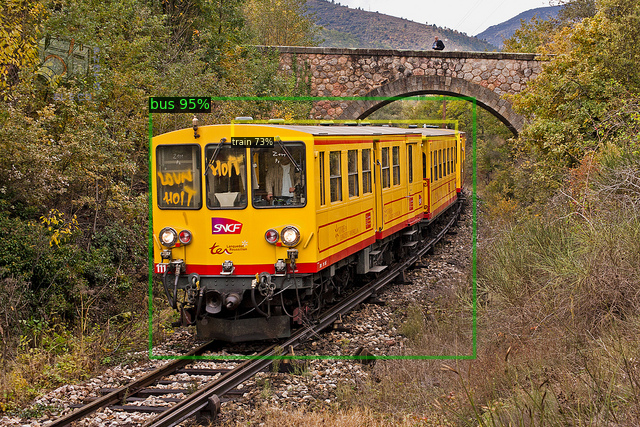
\includegraphics[width=\textwidth, height=0.17\textheight]{./../../final_results/Coco/COCO_test2014_000000006499_1shot.png}
  % }
  \subcaption{1-shot}
  \end{minipage}
  %
  \begin{minipage}{0.33\textwidth}
  % \fbox{
  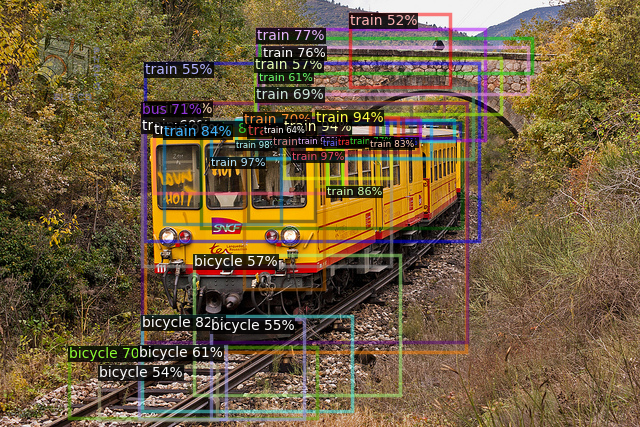
\includegraphics[width=\textwidth, height=0.17\textheight]{./../../final_results/Coco/COCO_test2014_000000006499_5shot.png}
  % }
  \subcaption{5-shot}
  \end{minipage}
  %
  \begin{minipage}{0.31\textwidth}
  % \fbox{
  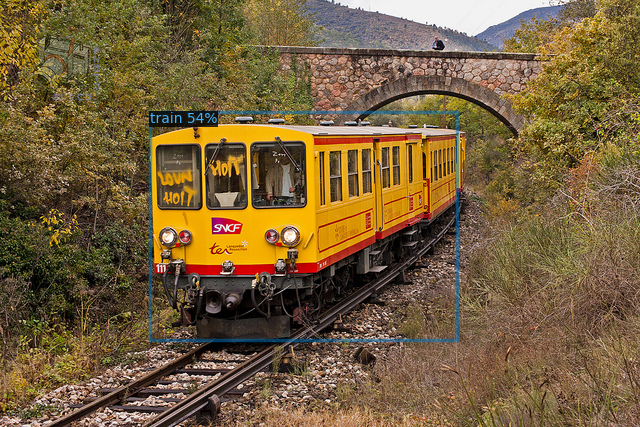
\includegraphics[width=\textwidth, height=0.17\textheight]{./../../final_results/Coco/COCO_test2014_000000006499_10shot.png}
  % }
  \subcaption{10-shot}
  \end{minipage}
  \caption{Detection Results on COCO dataset. }
  \label{coco_results}
\end{figure}


\begin{figure}[h!]
  \centering
  \begin{minipage}{0.33\textwidth}
  % \fbox{
  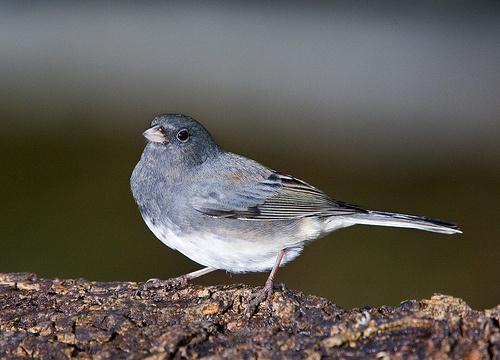
\includegraphics[width=\textwidth, height=0.17\textheight]{./../../final_results/Pascal/000148_1shot.png}
  % }
  \subcaption{1-shot}
  \end{minipage}
  %
  \begin{minipage}{0.33\textwidth}
  % \fbox{
  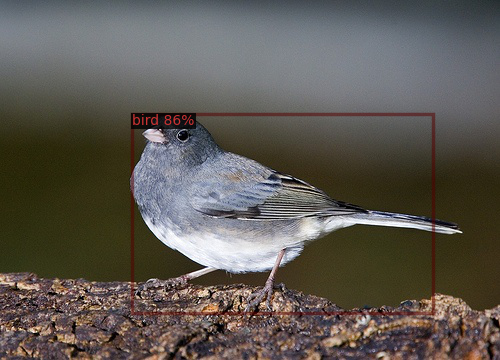
\includegraphics[width=\textwidth, height=0.17\textheight]{./../../final_results/Pascal/000148_5shot.png}
  % }
  \subcaption{5-shot}
  \end{minipage}
  %
  \begin{minipage}{0.31\textwidth}
  % \fbox{
  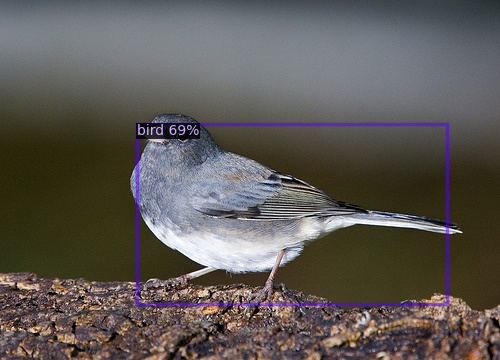
\includegraphics[width=\textwidth, height=0.17\textheight]{./../../final_results/Pascal/000148_10shot.png}
  % }
  \subcaption{10-shot}
  \end{minipage}
  \caption{Detection Results on PASCAL dataset. }
  \label{pascal_results}
\end{figure}


\begin{figure}[h!]
  \centering
  \begin{minipage}{0.33\textwidth}
  % \fbox{
  \includegraphics[width=\textwidth, height=0.17\textheight]{Kitti_1shot.png}
  % }
  \subcaption{1-shot}
  \end{minipage}
  %
  \begin{minipage}{0.33\textwidth}
  % \fbox{
  \includegraphics[width=\textwidth, height=0.17\textheight]{Kitti_5shot.png}
  % }
  \subcaption{5-shot}
  \end{minipage}
  %
  \begin{minipage}{0.31\textwidth}
  % \fbox{
  \includegraphics[width=\textwidth, height=0.17\textheight]{Kitti_10shot.png}
  % }
  \subcaption{10-shot}
  \end{minipage}
  \caption{Detection Results on KITTI dataset. }
  \label{kitti_plots}
\end{figure}

\begin{figure}[h]
  % \centering
  \begin{minipage}{0.47\textwidth}
  % \fbox{
  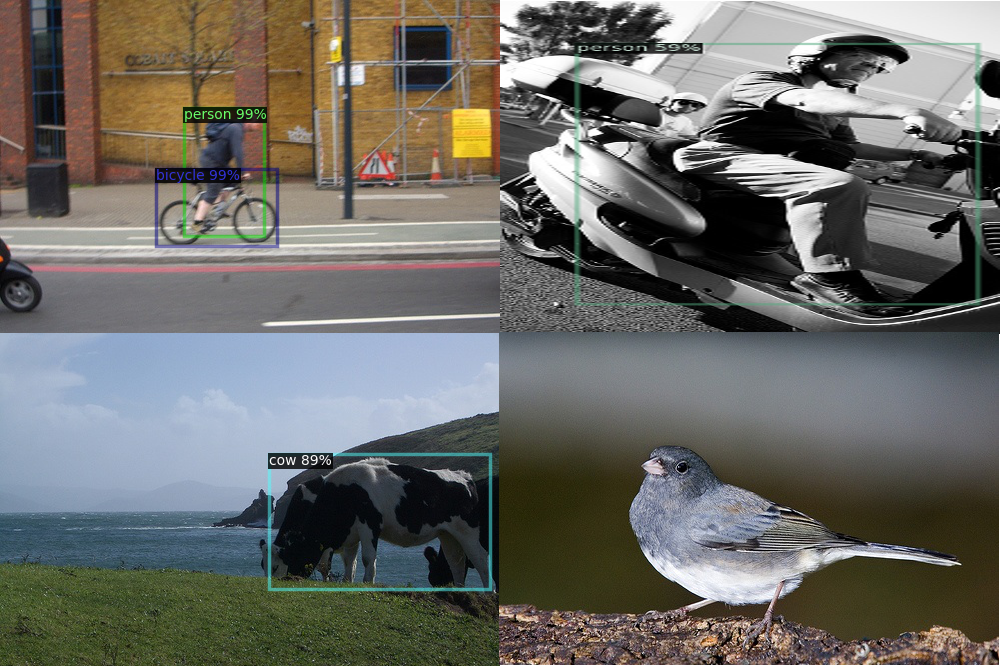
\includegraphics[width=\textwidth, height=0.17\textheight]{./../../figures/1shotpascal.png}
  % }
  \end{minipage}
  %
  \begin{minipage}{0.47\textwidth}
  % \fbox{
  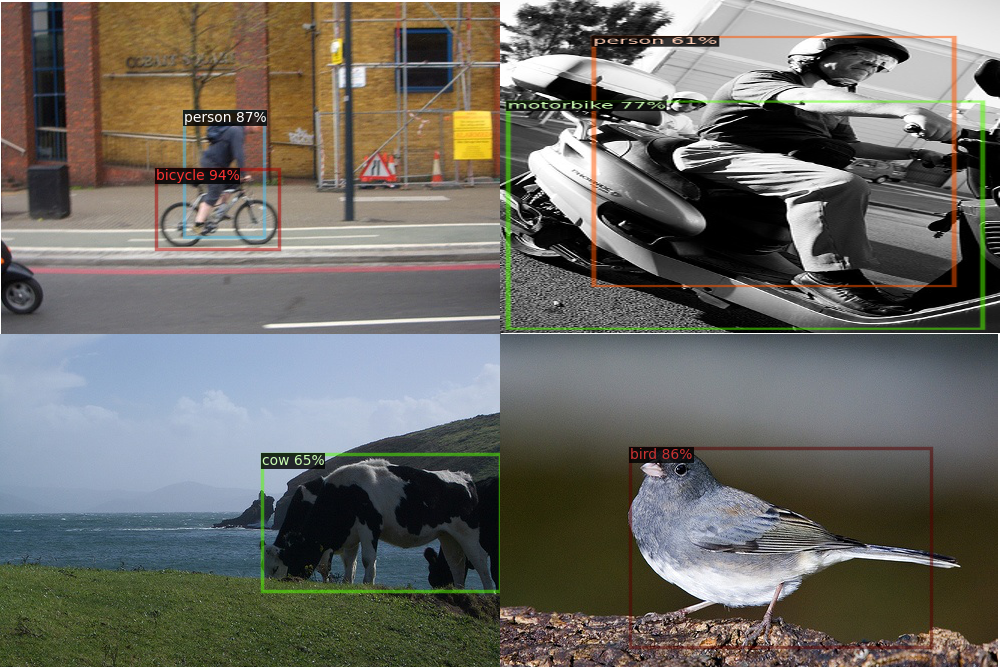
\includegraphics[width=\textwidth, height=0.17\textheight]{./../../figures/5shotpascal.png}
  % }
  \end{minipage}
  %
  \begin{minipage}{0.47\textwidth}
  % \fbox{
  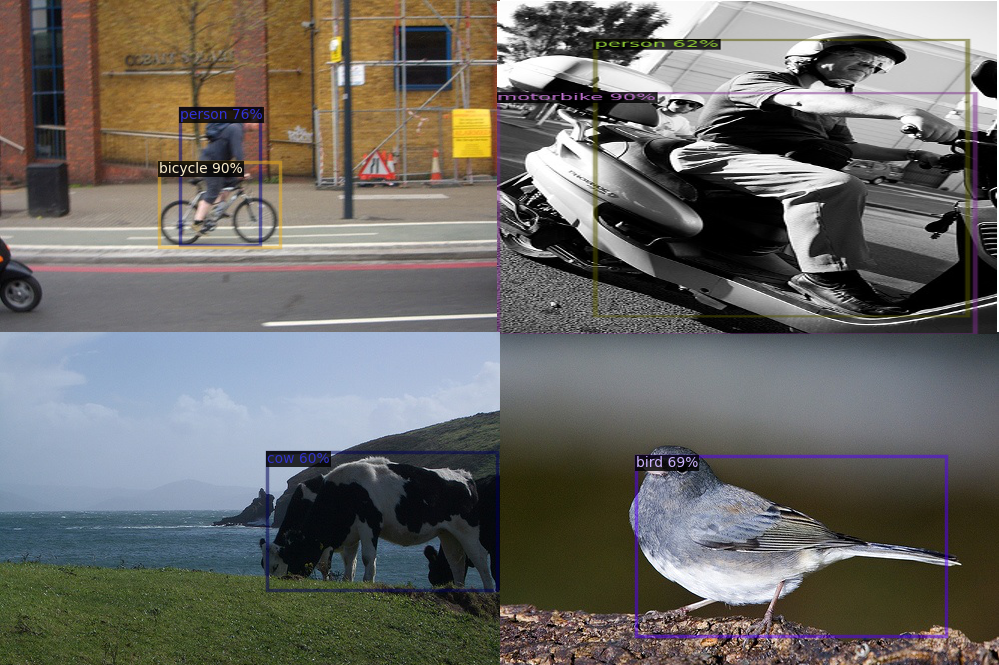
\includegraphics[width=\textwidth, height=0.17\textheight]{./../../figures/10shotpascal.png}
  % }
  \end{minipage}
  \caption{Our Results on the PASCAL Dataset }
  \label{finetuning}
\end{figure}


\begin{figure}[h]
  % \centering
  \begin{minipage}{0.47\textwidth}
  % \fbox{
  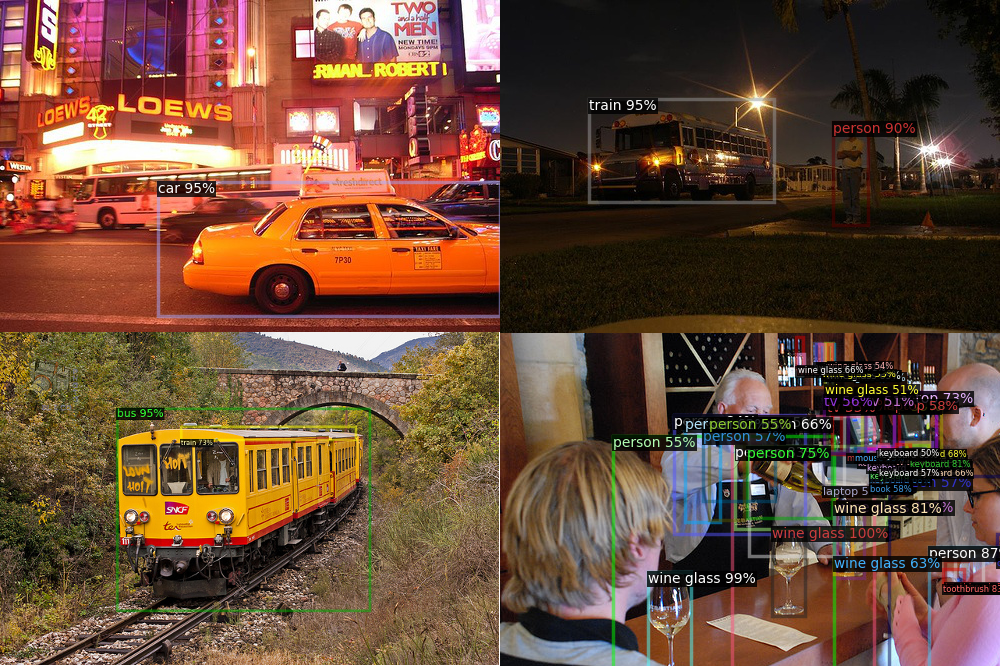
\includegraphics[width=\textwidth, height=0.17\textheight]{./../../figures/1shot.png}
  % }
  \end{minipage}
  %
  \begin{minipage}{0.47\textwidth}
  % \fbox{
  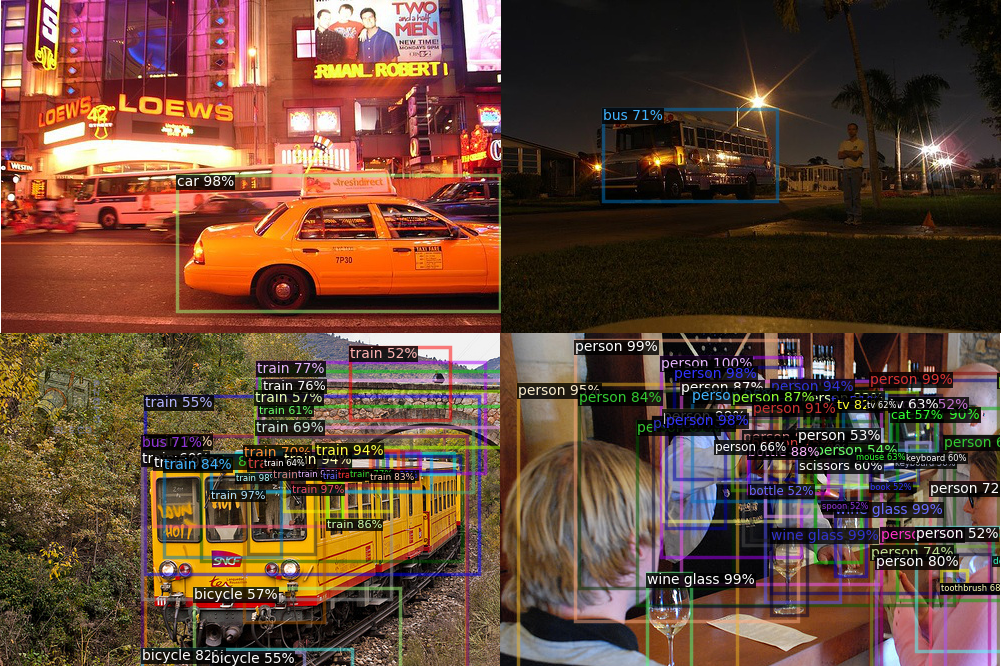
\includegraphics[width=\textwidth, height=0.17\textheight]{./../../figures/5shot.png}
  % }
  \end{minipage}
  %
  \begin{minipage}{0.47\textwidth}
  % \fbox{
  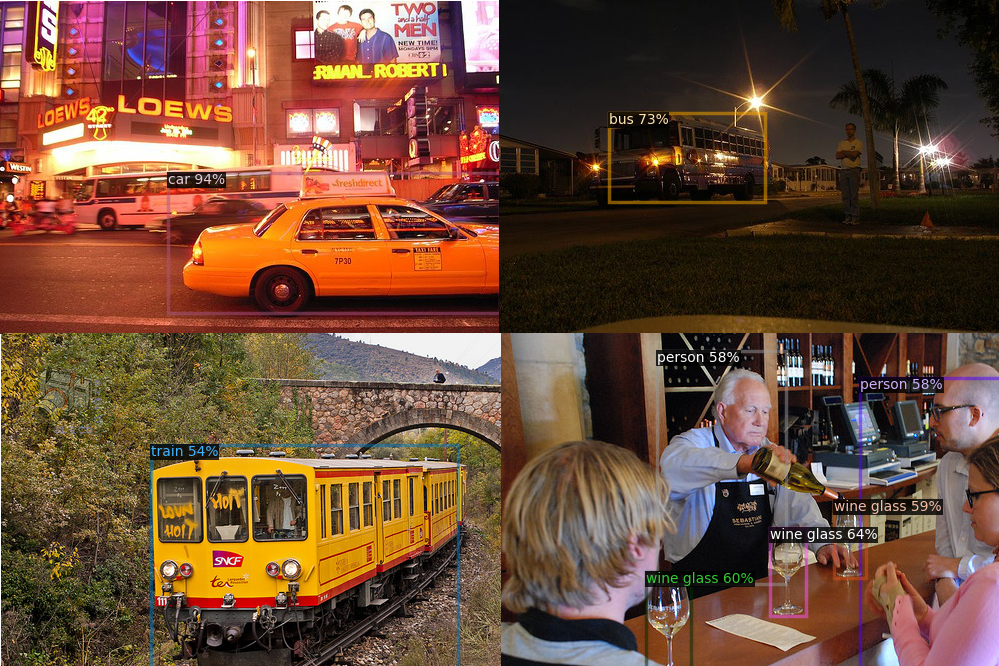
\includegraphics[width=\textwidth, height=0.17\textheight]{./../../figures/10shot.png}
  % }
  \end{minipage}
  \caption{Our Results on the COCO Dataset }
  \label{finetuning}
\end{figure}

\begin{figure}[h]
  % \centering
  \begin{minipage}{0.47\textwidth}
  % \fbox{
  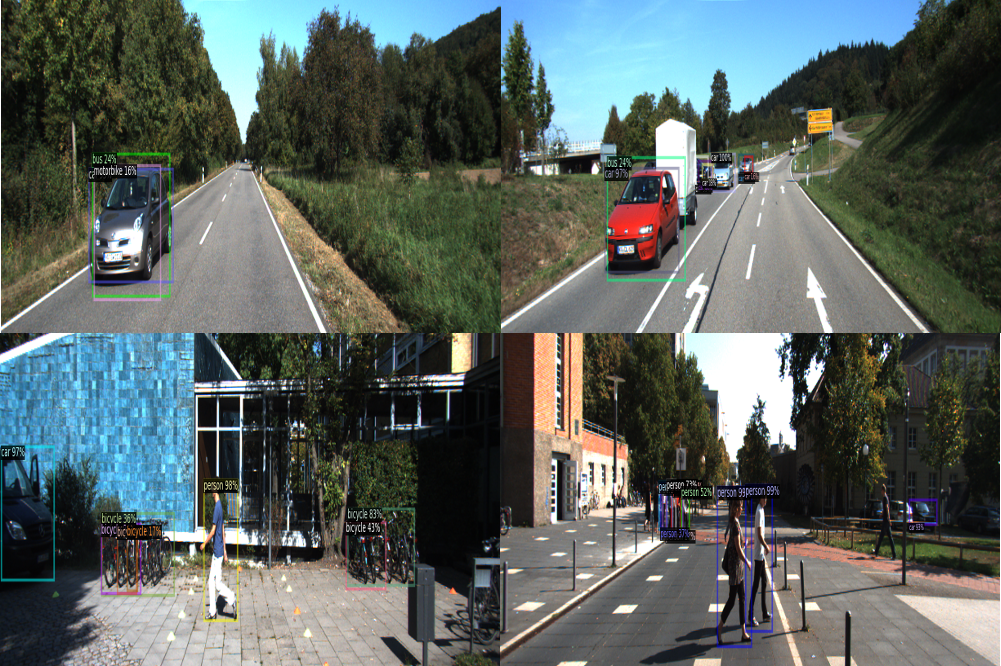
\includegraphics[width=\textwidth, height=0.17\textheight]{./../../figures/1shotkitti.png}
  % }
  \end{minipage}
  %
  \begin{minipage}{0.47\textwidth}
  % \fbox{
  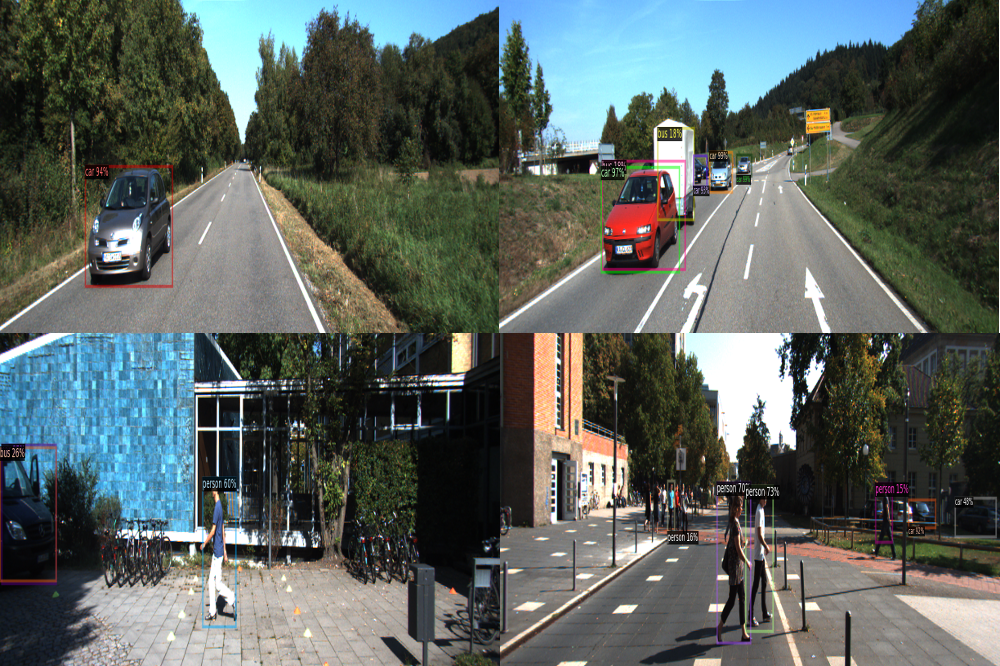
\includegraphics[width=\textwidth, height=0.17\textheight]{./../../figures/5shotkitti.png}
  % }
  \end{minipage}
  %
  \begin{minipage}{0.47\textwidth}
  % \fbox{
  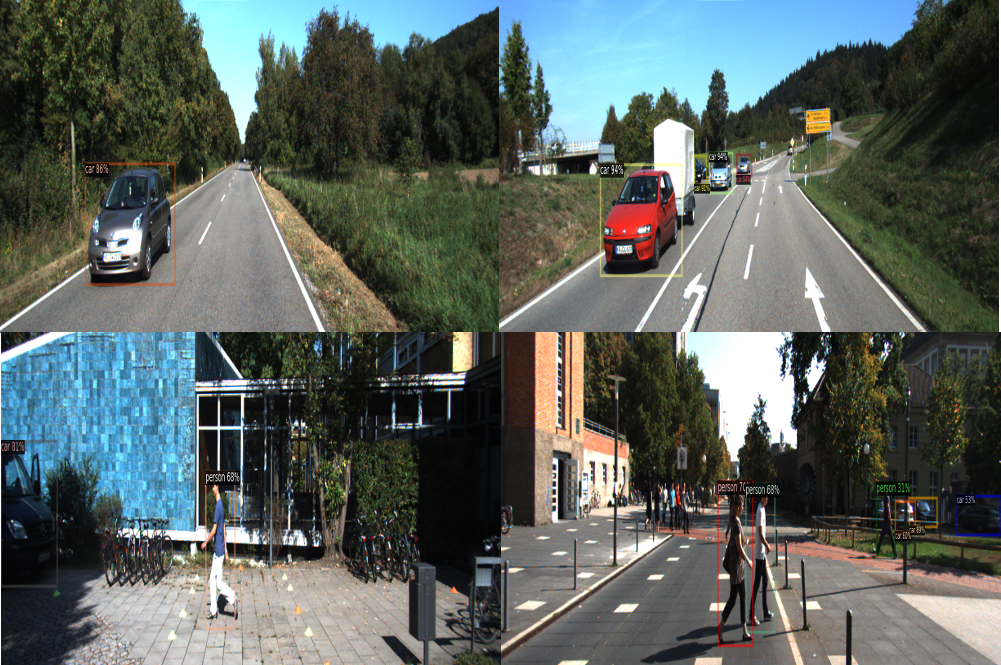
\includegraphics[width=\textwidth, height=0.17\textheight]{./../../figures/10shotkitti.png}
  % }
  \end{minipage}
  \caption{Our Results on the KITTI Dataset }
\end{figure}

\section{Conclusion}



\if{ %This is to remove the proposal from output
\section{Problem Statement}
A small child visiting a zoo with parents for the first time recognizes a strange animal---a zebra, 
she is told. She keeps walking and a few minutes later, by the infirmary, she recognizes another animal,
only smaller and wobbly this time. ``A baby zebra'', she exclaims. From just this one example, 
she will be able to recognize just about every zebra she will ever see. Not only this, 
she will also be able to make remarkable connections to other animal that are are similar 
to zebras \cite{samuelson2005they}. 

This is an ability machines have yet to acquire. Although machines have surpassed humans in 
visually recognizing objects, they still lack the ability to do so from a few examples. 
Recently,there have been promising advances towards the goal of making machines generalize 
from a few examples via a deep learning method called \textit{few-shot learning}. 
There are many important applications that could benefit from the ability to learn from a few 
samples. Like any other problem, there are various approaches to this this task.
In this project, we propose to evaluate and analyze two of the most promising approaches. 

Few-shot learning has received significant interest in the past few years, 
but mainly for the tasks of classification and rarely for object detection. 
In computer vision, the task of object detection is more challenging since the detector 
not only has to perform recognition of the different kinds of objects present,
it also has to localize them. This is already a challenging task that relies heavily 
on the availability of massive amounts of labeled training data. Now when a new data-point 
is obtained belonging to a novel category, adapting the model becomes a very difficult 
task especially when the new category contains a few samples. Recently, meta learning techniques 
have been proposed for adapting deep models to novel categories. However, they are not easily 
extendable to the task of object detection. Take for example the Matching \cite{VinyalsBLKW16} 
and Prototypical Networks \cite{snell2017prototypical}, building prototypes of objects is 
much more difficult than building prototype of the categories. Another approach that is being 
explored by researchers is to provide ways to fine-tune the detection layers of 
deep models to adapt to the new categories \cite{wang2020frustratingly}.

In this project we aim to do a comparative study of meta-learning and fine-tuning approaches 
towards object detection. We aim to experiment on benchmark datasets such as 
COCO \cite{LinMBHPRDZ14} and PASCAL \cite{Everingham10} and also extend these approaches 
towards 3D object detection with the KITTI dataset \cite{Geiger2013IJRR}.

In addition, we plan on examining how many shots are necessary to reach comparable accuracy relative to 
conventional detection approaches. To this end, we will attempt to develop a metric that assesses
the model's knowledge, and requests additional labeled examples if it has not reached a certain accuracy. 
This will allow us to further compare the performance of the two approaches. 

\section{Work Plan}

We plan to work on the meta-learning and fine-tuning based approaches simultaneously. 
Sayak and Bernard will focus on meta-learning-based approaches, while Om, Chetan and Vikarn will work 
on fine-tuning approaches. The experimental results will be compiled by Om and Vikarn while Sayak, 
Bernard and Chetan will work on final report compilation. 
}
\fi 



\appendix 
\section{More Results}



















\bibliographystyle{IEEEtran}
\bibliography{References}


\end{document}

